% Created 2022-07-11 Mon 14:43
% Intended LaTeX compiler: pdflatex
\documentclass[11pt]{article}
\usepackage[utf8]{inputenc}
\usepackage[T1]{fontenc}
\usepackage{graphicx}
\usepackage{longtable}
\usepackage{wrapfig}
\usepackage{rotating}
\usepackage[normalem]{ulem}
\usepackage{amsmath}
\usepackage{amssymb}
\usepackage{capt-of}
\usepackage{hyperref}
\author{Anak Wannaphaschaiyong}
\date{\today}
\title{Ec2 Note}
\usepackage{biblatex}

\begin{document}

\maketitle
\tableofcontents


\section{References}
\label{sec:org6c103f0}
\begin{itemize}
\item ref
\begin{itemize}
\item \href{https://medium.com/swlh/launch-and-manage-ec2-instances-using-aws-cli-7efae00e264b}{Launch and Manage EC2 Instances Using AWS CLI}
\item \href{https://docs.aws.amazon.com/cli/latest/userguide/cli-services-ec2-keypairs.html\#cli-services-ec2-keypairs-prereqs}{creating displaying, and deleting Amazon EC2 key pairs}
\end{itemize}
\end{itemize}
\section{blog\hfill{}\textsc{blog}}
\label{sec:org423743a}
\subsection{Using Terraform to set up ec2 instances for data science projects.\hfill{}\textsc{terraform}}
\label{sec:org0b9500a}
\subsubsection{Take Away}
\label{take-away}
\begin{itemize}
\item you will learn how to automate ec2 setup using terraform that is
suited for data science project.
\end{itemize}

\subsubsection{Tools}
\label{tools}
\begin{itemize}
\item EC2
\item Terraform
\end{itemize}
\subsubsection{Requirements}
\label{requirements}
\begin{enumerate}
\item Knowledge Requirements
\label{knowledge-requirements}
\begin{itemize}
\item understand basic of how to create terraform project
\item understand basic of how to set up ec2 instances
\end{itemize}

\item System Requirements
\label{system-requirements}
\begin{itemize}
\item WSL/Ubuntu

\begin{itemize}
\item I have only tested this in WSL
\end{itemize}

\item install all dependencies of cuda

\begin{itemize}
\item for list of software requirements, see

\begin{itemize}
\item \url{https://www.tensorflow.org/install/gpu\#linux\_setup}
\end{itemize}
\end{itemize}

\item optional

\begin{itemize}
\item Docker \# References
\end{itemize}

\item Terraform AWS documentation

\begin{itemize}
\item \url{https://registry.terraform.io/providers/hashicorp/aws/latest/docs/resources/instance\#availability\_zone}
\end{itemize}

\item pytorch docker image

\begin{itemize}
\item \url{https://github.com/anibali/docker-pytorch} \# Content
\end{itemize}
\end{itemize}
\end{enumerate}

\subsubsection{Code}
\label{code}
\begin{enumerate}
\item AWS
\label{aws}
\begin{enumerate}
\item export the following environment variables including

\begin{itemize}
\item AWS\textsubscript{ACCESS}\textsubscript{KEY}\textsubscript{ID}
\item AWS\textsubscript{SECRET}\textsubscript{ACCESS}\textsubscript{KEY}
\item AWS\textsubscript{DEFAULT}\textsubscript{REGION}
\end{itemize}
\end{enumerate}

\item Terraform
\label{terraform}
\begin{enumerate}
\item create terraform project
\item In the project, create main.tf and copy\&paste the following code
\end{enumerate}

\begin{verbatim}
    resource "aws_instance" "web" {
      ami = "ami-08962a4068733a2b6"
      instance_type = "p3.8xlarge"
      cpu_core_count = 16
      cpu_threads_per_core = 2
      tags = {
        Name = "HelloWorld"
      }

    }
\end{verbatim}

\begin{enumerate}
\item now you have ec2 running with
\end{enumerate}
\end{enumerate}
\subsection{A Note of X where X = AWS EC2 services.}
\label{sec:org4aa7dbf}
An EC2 instance has 4 state of life cycle: running, stopped, and terminated. Furthermore, state transition (or action) of an EC2 instance is launch, rebooting, pending, shutting-down, and stopping, see

\begin{figure}[htbp]
\centering
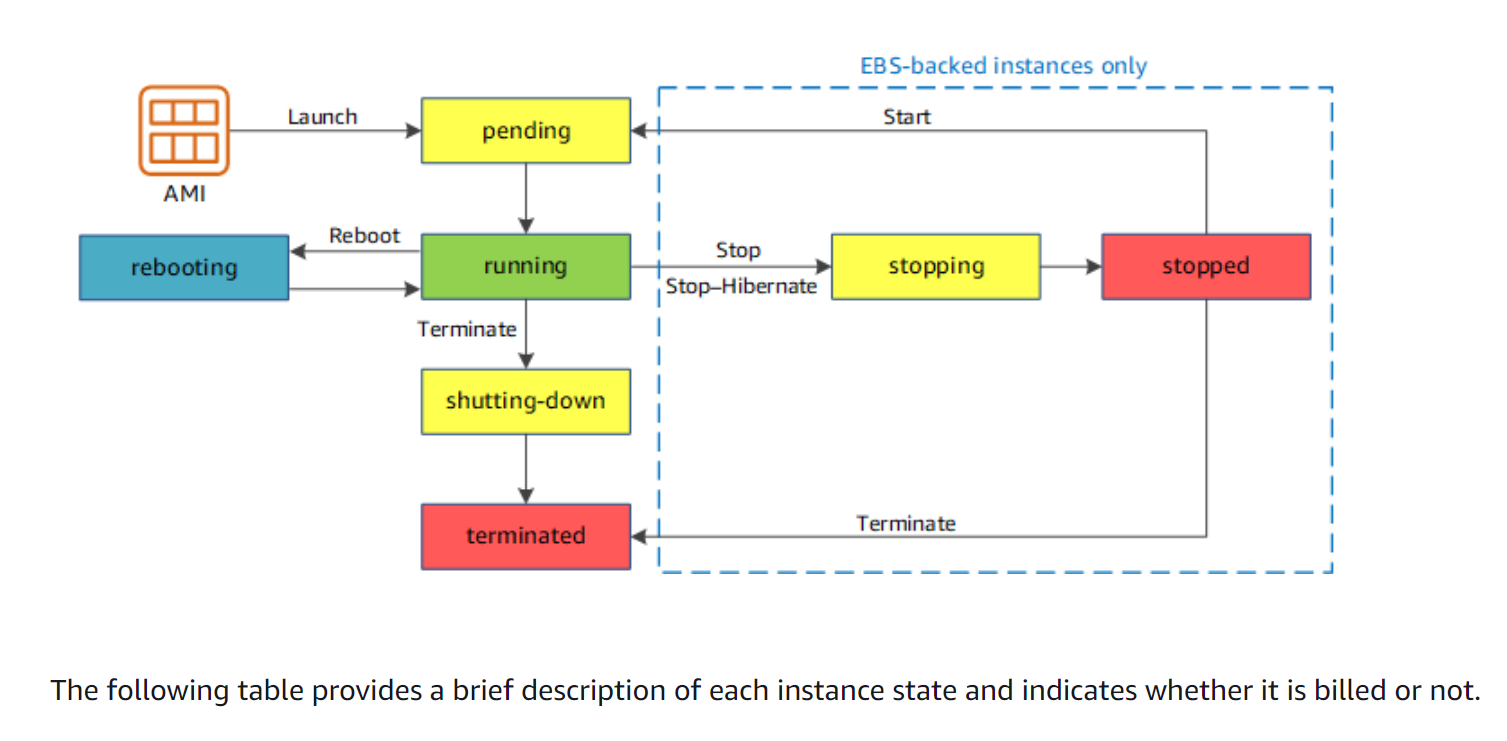
\includegraphics[width=.9\linewidth]{./images/screenshot_20220711_141153.png}
\caption{\label{ec2_life_cycle}EC2 instance life cycle}
\end{figure}

Illustrate EC2 instance life cycle using state and state-transition ()
To launch EC2 from command line, write \textasciitilde{}\textasciitilde{}

\section{command line}
\label{sec:org4440227}
\subsection{start instances}
\label{sec:orgefa1e4d}
\texttt{aws ec2 start-instances -{}-instance-ids i-04857a8be9b9de952}
\subsection{create security-group}
\label{sec:org7450afc}
\texttt{aws ec2 create-security-group -{}-group-name "expert-crypto" -{}-description "expert discovery for crypto"}
\subsection{create key-value pair}
\label{sec:org43eebeb}
\texttt{aws ec2 create-key-pair -{}-key-name <your key name>}
\subsection{create new EC2 instance}
\label{sec:org55f8bbc}
\texttt{aws ec2 run-instances -{}-image-id ami-0fb653ca2d3203ac1 -{}-instance-type t2.micro -{}-count 1 -{}-security-group-ids sg-0db2887fa3dbd0493 -{}-key-name ExpertCrypto}
\subsection{create tags for resources}
\label{sec:org7e732fc}
\texttt{aws ec2 create-tags -{}-resources i-07f6b9c46c87b4233 -{}-tags Key=test,Value=test}
\end{document}
